%%%%%%%%%%%%%%%%%%%%%%%%%%%%%%%%%%%%%%%%%
% University Assignment Title Page 
% LaTeX Template
% Version 1.0 (27/12/12)
%
% This template has been downloaded from:
% http://www.LaTeXTemplates.com
%
% Original author:
% WikiBooks (http://en.wikibooks.org/wiki/LaTeX/Title_Creation)
%
% License:
% CC BY-NC-SA 3.0 (http://creativecommons.org/licenses/by-nc-sa/3.0/)
% 
% Instructions for using this template:
% This title page is capable of being compiled as is. This is not useful for 
% including it in another document. To do this, you have two options: 
%
% 1) Copy/paste everything between \begin{document} and \end{document} 
% starting at \begin{titlepage} and paste this into another LaTeX file where you 
% want your title page.
% OR
% 2) Remove everything outside the \begin{titlepage} and \end{titlepage} and 
% move this file to the same directory as the LaTeX file you wish to add it to. 
% Then add \input{./title_page_1.tex} to your LaTeX file where you want your
% title page.
%
%%%%%%%%%%%%%%%%%%%%%%%%%%%%%%%%%%%%%%%%%

%----------------------------------------------------------------------------------------
%	PACKAGES AND OTHER DOCUMENT CONFIGURATIONS
%----------------------------------------------------------------------------------------

\documentclass[a4paper]{report}
\usepackage[utf8]{inputenc}
\usepackage{imakeidx}
\makeindex[columns=5, title=Alphabetical Index, intoc ]
   
\usepackage[usenames,dvipsnames]{color}

\usepackage[hyperfootnotes=false]{hyperref}
\hypersetup{
 colorlinks=false,
 citecolor=black,
 linkcolor=Red,
 urlcolor=black}

 
\usepackage{lipsum}
\usepackage{fancyhdr}
\usepackage{xcolor}

\usepackage{etoolbox}

\usepackage{scrextend}
\changefontsizes[16pt]{14pt}

\makeatletter
\patchcmd{\@fancyhead}{\rlap}{\color{black}\rlap}{}{}
\patchcmd{\headrule}{\hrule}{\color{black}\hrule}{}{}
\patchcmd{\@fancyfoot}{\rlap}{\color{black}\rlap}{}{}
\patchcmd{\footrule}{\hrule}{\color{black}\hrule}{}{}
\makeatother

\usepackage[italian]{babel}
\usepackage[utf8]{inputenc}
\usepackage{fancyhdr}
 
\pagestyle{fancy}
\makeatletter
\newcommand*{\rom}[1]{\expandafter\@slowromancap\romannumeral #1@}
\makeatother


\usepackage{caption}
\usepackage{graphicx}

\usepackage{lipsum}
\usepackage{fancyhdr}
\usepackage{xcolor}

\usepackage{etoolbox}
 
\usepackage{color}   %May be necessary if you want to color links

\usepackage{mathptmx}
\usepackage{anyfontsize}
\usepackage{t1enc}

\usepackage{hyperref}
\hypersetup{
    colorlinks=true, %set true if you want colored links
    linktoc=all,     %set to all if you want both sections and subsections linked
    linkcolor=black,  %choose some color if you want links to stand out
}

\makeatletter
\let\@orig@endthebibliography\endthebibliography
\renewcommand\endthebibliography{%
  \xdef\@kept@last@number{\the\c@enumiv}%
  \@orig@endthebibliography}

\newenvironment{thesitography}[1]
  {\def\bibname{Siti consultati}%
   \thebibliography{#1}%
   \setcounter{enumiv}{\@kept@last@number}%
}
  {\@orig@endthebibliography}
\makeatother

\renewcommand{\rmdefault}{ptm}

\usepackage{url}

\usepackage{wrapfig}

\makeatletter
\g@addto@macro{\UrlBreaks}{\UrlOrds}
\makeatother

\begin{document}

\begin{titlepage}

\newcommand{\HRule}{\rule{\linewidth}{0.5mm}} % Defines a new command for the horizontal lines, change thickness here

\newcommand{\HRulea}{\rule{\linewidth}{0.5mm}} % Defines a new command for the horizontal lines, change thickness here

\newcommand{\HRuleb}{\rule{\linewidth}{0.7mm}} % Defines a new command for the horizontal lines, change thickness here

\newcommand{\newlecture}{%
  \clearpage
  \refstepcounter{lecture}%
  \noindent{\large\bfseries \lecturename{} \thelecture}%
  \par\bigskip\noindent\ignorespaces%
}

\renewcommand{\sectionmark}[1]{\markright{#1}}

\renewcommand{\familydefault}{\rmdefault}

\center % Center everything on the page
 
%----------------------------------------------------------------------------------------
%	HEADING SECTIONS
%----------------------------------------------------------------------------------------

\textsc{\LARGE Alma Mater Studiorum}\\[0.2cm] % Name of your university/college
\textsc{\LARGE Universit\'a degli studi di}\\[0.2cm] % Name of your university/college
\textsc{\LARGE Bologna}\\[0.1cm]
\HRulea \\[0.0cm]
\HRuleb \\[0.5cm]
\textsc {\textbf{\LARGE Scuola di Scienze}}\\[0.5cm] % Major heading such as course name
\textsc{\textit{\Large Corso di Laurea in Informatica}}\\[0.5cm] % Minor heading such as course title
%\begin{figure}[h]
%\includegraphics[scale=0.3]{/home/tonino/Desktop/Tesi/image/unibo.jpg}\centering
%\end{figure}

%----------------------------------------------------------------------------------------
%	TITLE SECTION
%----------------------------------------------------------------------------------------

\HRule \\[0.4cm]
{ \huge \bfseries Studio e realizzazione}\\[0.4cm] % Title of your document
{ \huge \bfseries di un'applicazione per il}\\[0.4cm] % Title of your document
{ \huge \bfseries Marketing di prossimit\'a}\\[0.4cm] % Title of your document
\HRule \\[1cm]
 
%----------------------------------------------------------------------------------------
%	AUTHOR SECTION
%----------------------------------------------------------------------------------------

\begin{minipage}[t]{5cm}
	\begin{flushleft} \Large
		\emph{ \bfseries Relatore:} \\
		Chiar.mo Prof. \\ Luciano \textsc{Bononi} % Supervisor's Name
		\\[0.1cm] % Your name

		\emph{ \bfseries Correlatore:} \\
		Dott. Luca \textsc{Bedogni} % Supervisor's Name
	\end{flushleft}

\end{minipage}
~
\begin{minipage}[t]{5cm}
	\begin{flushright} \Large
		\emph{ \bfseries Candidato:}\\
		Alessandro \textsc{Panipucci}\\[0.1cm]
	\end{flushright}
	
\end{minipage}\\[1cm]

%----------------------------------------------------------------------------------------
%	DATE SECTION
%----------------------------------------------------------------------------------------
\HRule \\[0.2cm]

{ \bfseries \textsc \textbf \large \rom{2} {Sessione}\\[0.2cm]
	 Anno Accademico 2014/2015}

%----------------------------------------------------------------------------------------
%	LOGO SECTION
%----------------------------------------------------------------------------------------

\vfill % Fill the rest of the page with whitespace

\end{titlepage}

\pagestyle{fancy}
\makeatletter
\newcommand{\unchapter}[1]{%
  \begingroup
  \let\@makechapterhead\@gobble % make \@makechapterhead do nothing
  \chapter{#1}
  \endgroup
}
\makeatother
\chapter*{Introduzione}
\markboth{Introduzione}{}
\addcontentsline{toc}{chapter}{Introduzione}
\vspace{4em}


Il marketing di prossimitá (proximity marketing) é una tecnica di marketing che opera su un'area geografica delimitata e precisa attraverso tecnologie di comunicazione di tipo visuale e mobile con lo scopo di promuovere la vendita di prodotti e servizi.\\[0.2cm]

Questa tecnica di marketing non agisce su un target di utenti ben definito, bensí sugli individui che si trovano in una determinata area e siano in prossimitá di un dispositivo attraverso il quale sia possibile instaurare una comunicazione; si tratta quindi di una modalitá moderna della distribuzione di volantini pubblicitari cartacei che, trasformati in materiale digitale, possono diventare interattivi tramite gli apparati di proximity marketing più evoluti come il (RFID, NFC, QrCode, audio di prossimitá, motion capture, eye tracking, iBeacon).
Il proximity marketing puó trovare applicazione in molti contesti, come ad esempio nei cinema (programmazione, trailer, messaggi pubblicitari), centri commerciali (buoni sconto, descrizione dei prodotti), negozi di giochi (giochi Java/Flash per cellulare), fiere (mappe degli stand, agenda degli eventi, business card dei relatori), concerti (suonerie, video musicali), tourist information access point (informazioni varie).\\[0.2cm]

La tesi propone uno strumento che applica questo concetto ai
viaggi turistici, mettendo a disposizione degli utenti dei percorsi, composti da obiettivi (le pietre miliari dell’itinerario) e creati da operatori convenzionati (quali aziende, associazioni o altri soggetti), al termine dei quali potranno essere vinti premi (sconti, omaggi, . . . ) se verrá data prova di aver attraversato gli obiettivi richiesti.
Ai giorni d'oggi il mondo è dominato dagli smartphone e quindi l'importanza di una strategia che ne sfrutti le potenzialitá é evidente, dato che essa puó essere in grado di “effettuare attivitá promozionali e informative al cliente che si trova vicino o all’interno del negozio nel momento in cui é disposto ad acquistare” \cite{rif1} e,inoltre, buone campagne di marketing di prossimitá possono valorizzare il brand aziendale e favorire sponsor e investimenti \cite{rif4}.\\[0.2cm]

Lo scenario d'uso tipico riguarda specialmente chi seguirá il percorso come intrattenimento durante il proprio periodo di vacanza, incentivato dalla consapevolezza che al termine dell’itinerario otterrà un qualche forma di premio recandosi nel negozio dell'azienda, ma questo non é l’unico scenario possibile. Un operatore infatti puó creare i tragitti nel modo che preferisce, per esempio definendone uno che attraversa tutti i suoi negozi o un loro sottoinsieme oppure creare tragitti che percorrono tutta i monumenti di maggiore importanza della località e tra questi inserire il locale del tragitto dove poter ritirare il premio vinto.\\[0.2cm]

L'applicazione permette di aumentare il bacino della propria clientela semplicemente creando un tragitto e mettendo in palio un premio, rendendone l'esperienza allo stesso tempo divertente ed economicamente vantaggiosa per il cliente. Infatti, come scrive Sciortino, “applicare strategie volte ad attrarre e fidelizzare un cliente/visitatore attraverso logiche ludiche in un contesto per sua natura non propriamente gaming, [ . . . ] porta il pubblico a cambiare il proprio atteggiamento da consumatore a protagonista della propria esperienza” \cite{rif5}.\\[0.2cm]

Ad oggi ci sono diverse applicazione con caratteristiche simili , discusse nel capitolo 1 , ma nessuna permette agli operatori di creare i propri percorsi totalmente personalizzati a cui associare precisi premi.

\renewcommand*\contentsname{Indice}
\tableofcontents

\chapter{Stato dell'arte}

In un’epoca caratterizzata dal grande sviluppo delle applicazioni Mobile il cellulare smartphone oggi è uno strumento fondamentale quando si viaggia, non solo per telefonare ai parenti ma soprattutto per gestire il proprio viaggio tramite le diverse applicazioni che facilitano tantissimo la ricerca dei posti migliori , rendendo sempre più diffuso il cosiddetto marketing di prossimità.\\

La tecnologia sta cambiando tempi e tendenze dato che sempre più brand si stanno muovendo verso questa direzione approfittando del “nuovo potere promozionale” per raggiungere i propri clienti e coinvolgerli in un’esperienza pubblicitaria più evoluta.\\

Infatti i grandi brand scelgono il marketing di prossimità in quando aumenta il tasso di conversione perciò come dice Nedim Bali, Marketing Manager di McDonald Turchia:\\
“Noi di McDonald amiamo sorprendere e soddisfare i nostri clienti, non solo attraverso un buon cibo e l’ottimo rapporto di qualità/prezzo ma anche, migliorando l’esperienza d’acquisto grazie all’utilizzo di nuove tecnologie”.\cite{rif9}\\
I numeri parlano chiaro:
McDonald ha aumentato del 20\% il suo tasso di conversione sfruttando la tecnologia di marketing di prossimità all’interno di 15 McCaffè situati ad Instambul, in Turchia.\\ Il 30\% degli utenti che hanno ricevuto l’offerta l’hanno sfruttata più volte tornando spesso all’interno del punto vendita. Questi dati sono stati raccolti in tempo reale, nel momento in cui il consumatore ha eseguito l’azione: è anche per questo che i grandi brand scelgono il marketing di prossimità.\\
Passiamo al caso Carrefour, un’azienda molto conosciuta nel settore della grande distribuzione o GDO, che come McDonald ha scelto la tecnologia di proximity marketing ottenendo dei risultati molto positivi.\\
Il coinvolgimento degli utenti, all’interno del supermercato, è aumentato del 400\% grazie all’utilizzo di un’app mobile che ha alimentato le vendite e semplificato l’esperienza tra gli scaffali.\\[0.2cm]

Al giorno d'oggi è diventato sempre più comune vedere nuove applicazioni e nuovi modi di interagire con tutto ciò che ci circonda.\\
Una di queste è iBeacon, nome che deriva dalla parola beacon, faro, è un sistema di proposta contestuale di contenuti basati su microgeolocalizzazione(beacons) su cui Apple ha deciso di puntare a discapito di NFC.\\
I beacons non sono nient’altro che piccoli trasmettitori bluetooth tramite i quali è possibile avere un’interazione completamente nuova, mai vista prima sul mercato. Infatti, con i beacons l’interazione è completamente implicita: l’utente non ha idea di cosa avviene in background, semplicemente ciò avviene.\\
In poche parole iBeacon permette al negozio di inviare sull’applicazione un messaggio di benvenuto al cliente, una guida per utilizzare iBeacon in quel locale, un coupon di sconto speciale per acquistare alcuni capi, o simili.\\
Questa è solo una delle app che puntano sul marketing di prossimità , una delle più famose è TripAdvisor che aiuta nella pianificazione dei viaggi turistici mettendo a disposizione recensioni di altri viaggiatori e ancora Wimo Prox che consente agli utenti di geolocalizzare le attività commerciali a loro più vicine, visualizzando offerte e promozioni in abbinamento ad utili informazioni sul luogo, mappe ed informazioni turistiche.\\

Tra le app “classiche” va ricordata anche Fourquare che in viaggio aiuta nella ricerca di monumenti ,bar ,negozi ristoranti e da anche dei feedback e foto per far capire agli utenti se quel luogo è giusto per loro.\\

Altre app sono Cibando e Restopolis, che mettono in contatto i consumatori con le migliori attività locali grazie ai dettagli approfonditi e contenuti di qualità, adottano un avanzatissimo modello di distribuzione web: allargare la visione fuori dalla cerchia dei conoscenti, verso il virale, affidando la parola al content marketing, dove sono i contenuti a rappresentare la comunicazione.\\

Come si può sfruttare questa tecnologia e come si può farla utilizzare al maggior numero di persone possibile?\\
Nell'articolo di Denisi M. \cite{rif14} si ottiene la seguente risposta: “Il miglior modo per coinvolgere gli utenti è quello di fornire uno strumento semplice e di impatto che permetta di costruire qualcosa in maniera intuitiva.”\\

Queste applicazioni inoltre permettono a un'azienda di sapersi distinguere, il quale è fondamentale dato che per il 2016 si parla di investimenti in servizi di marketing di prossimità pari a 2.3 miliardi di dollari.\\


\chapter{Progettazione}

La tesi ha alcuni elementi fondamentali quali:\\[0.2cm]

\begin{itemize}  

\item \textsc{\bfseries Utenti} : \emph{Sono coloro che percorrono i tragitti, ne completano gli obiettivi e vincono i premi.}

\item \textsc{\bfseries Operatori} : \emph{Essi creano percorsi e obiettivi e ne stabiliscono i premi associati.}

\item \textsc{\bfseries Percorsi} : \emph{Sono gli itinerari creati dagli operatori a beneficio degli utenti. Essi sono costituiti da obiettivi da raggiungere, al completamento dei quali è prevista l’assegnazione di un premio.}

\item \textsc{\bfseries Obiettivi} : \emph{Sono le pietre miliari del percorso, attraverso cui gli utenti devono dare prova di essere passati per vincere i premi.}

\item \textsc{\bfseries Premi} : \emph{Consistono ad esempio in sconti e omaggi ed è a loro collegata una lista di obiettivi obbligatori (relativi a ogni percorso) che gli utenti devono attraversare per poterli vincere.}\\[0.2cm]

\end{itemize}
L'applicazione permette a utenti e operatori di registrarsi creando un account ed effettuare il login dopo l'avvenuta registrazione al fine di usare il servizio.\\
L'accesso può avvenire anche tramite Facebook allineando così l'app a tutte le altre preesistenti.\\
Inoltre è possibile ottenere i percorsi e tutte le informazioni a loro associate (cioè obiettivi, premi e operatore di appartenenza) in maniera geolocalizzata,
a seconda della modalià scelta infatti si potranno ottenere i percorsi vicini , consigliati o i percorsi di una determinata città e in aggiunta oltre a una illustrazione testuale sarà possibile anche visualizzare i percorsi su la mappa grazie all'utilizzo dei servizi di Google Maps.\\
Quest'ultima visualizzazione permette anch'essa di selezionare i percorsi , in modalità utente ,semplicemente cliccando su uno degli obiettivi del tragitto.\\[0.2cm]

Gli utenti possono dar prova di aver attraversato ogni singolo obiettivo inviando al server il codice assocciato che comunicherà se e quali premi sono stati vinti e le informazioni su tutti i percorsi che passano per l’obiettivo verificato.\\
In più i percorsi iniziati dall'utente vengono salvati in un'apposita activity per ricominciare il percorso successivamente senza perdere i progressi fatti fino a quel momento.\\ 
Una volta vinto un premio, gli utenti possono ottenerne il codice di riscossione (valido solamente entro un tempo limitato) tramite un’apposita operazione. Il codice deve poi
essere mostrato all’operatore a cui appartiene il premio, che ne verificherà la validità.\\[0.2cm]

Infine, sono dedicate agli operatori tutta una serie di funzionalità per creare, modificare ed eliminare percorsi e premi.\\
Gli obiettivi invece, una volta inseriti non sono più modificabili, poichè sono condivisi da tutti gli operatori.




\chapter{Implementazione}

\section{Login e Registrazione}

\vspace{2em}

\begin{wrapfigure}{L}{0.45\textwidth}
\centering
\includegraphics[width=0.4\textwidth]{./image/login.png}
\caption{\label{fig:login}Login activity}
\end{wrapfigure}

La prima activity nell'applicazione è quella del Login (figura 3.1) che permette all'utente di accedere ai servizi dell'app a seconda del login e password inserite.
La registrazione è possibile solo per quando riguarda l'utente e non per l'operatore in quando quest'ultimo può creare obiettivi , percorsi e premi , pertanto ha in mano una serie di operazioni sensibili.
Quindi si è pensato di evitare la registrazione dell'operatore sull'applicazione ma di permettere di ottenere l'account solo tramite acquisto o altra maniera di registrazione .

\begin{wrapfigure}{R}{0.45\textwidth}
\centering
\includegraphics[width=0.4\textwidth]{./image/Registrazione_utente.png}
\caption{\label{fig:login}Registrazione Utente}
\end{wrapfigure}

Mentre per la creazione di un'account utente (figura 3.2) si ha bisogno dei seguenti elementi:

\begin{itemize}  

\item \textsc{\bfseries Username} : nome univoco che identifica l'utente nell'applicazione .
\item \textsc{\bfseries Password} : è una sequenza di caratteri alfanumerici utilizzata per accedere in modo esclusivo. 
\item \textsc{\bfseries Conferma Password} : inserita per rendere consapevole l'utente della password inserita ed evitare che abbia commesso degli errori .
\item \textsc{\bfseries Tags} : sono i tipi di percorsi preferiti che l'utente sceglie in fase di registrazione.\\

\end{itemize}

Una volta compilato tutti gli elementi in fase di registrazione inserendo un username univoco e una password sicura di almeno otto caratteri con almeno una cifra e un carattere speciale e aver cliccato su invio l'utente ha in possesso un account che gli permetterà di usufruire dei servizi connessi a esso.\\
La sicurezza della password è controllata tramite l'utilizzo delle espressioni regolari.\\
Le espressioni regolari rappresentano uno strumento molto potente per lavorare sulle stringhe e possono essere utilizzate, sia per convalidare i dati, sia per effettuare ricerche all'interno di un testo.\\ 
La sintassi di questo pseudo-linguaggio è molto flessibile e consente di creare espressioni in base alle proprie esigenze.


\section{Due modalità per un app}

L'applicazione è l'unione di due modalità , quindi chi la usa può decidere se utilizzarla in modalità utente o in quella operatore.

\section{Utente}

\vspace{2em}

\begin{wrapfigure}{L}{0.45\textwidth}
\centering
\includegraphics[width=0.4\textwidth]{./image/navigation_fragment.png}
\caption{\label{fig:lato utente}lato utente }
\end{wrapfigure}

Quando si utilizza il lato utente l'obiettivo e svolgere i percorsi forniti dall'app al fine di ottenere i premi.\\[0.2cm]
Ci si può spostare da un'activity all'altra semplicemente cliccando sull'apposito bottone nella navigation fragment (figura 3.3).\\[0.2cm]
Il nome dei tasti della navigation fragment danno una breve descrizione dell'activity che mostreranno infatti se si sceglie "Home" l'utente utilizzerà il servizio vero e proprio , cioè la ricerca dei percorsi , mentre se la scelta è "Premi" l'app visualizzerà tutti i premi vinti fino a quel momento e non ancora scaduti o riscossi , e infine c'è "Percorsi" che permette di continuare i tragitti iniziati in precedenze e non conclusi senza perdere i "passi" in avanti fin lì fatti , rendendo l'app molto più appetibile.
\clearpage
\subsection{Visualizzazione}
\vspace{2em}
\begin{wrapfigure}{R}{0.45\textwidth}
\centering
\includegraphics[width=0.4\textwidth]{./image/mappa_Utente.png}
\caption{\label{fig:mappa utente}mappa utente}
\end{wrapfigure}
Se si cercano i percorsi bisogna cliccare sul tasto "Home"
che da due visualizazioni di ricerca , una testuale dove l'utente tramite un semplice swipe da destra verso sinistra può scegliere la modalità di ricerca dei percorsi più opportuna inoltre ognuno di quest'ultime hanno un loro 
colore caratteristico che rende più intuitiva la ricerca e la percezione della modalità in cui ci si trova , in più è stato aggiunto il nome del tipo di ricerca in cui ci si trova al di sopra della stessa.
Quindi le modalità che l'utente può utilizzare sono:\\[0.2cm]

\begin{itemize}  

\item \textsc{\bfseries Vicinanza} : i percorsi che vengono visualizzati sono quelli più vicini all'utente nel momento in cui fa la ricerca;\\
\item \textsc{\bfseries Consigliati} : i percorsi che vengono visualizzati sono quelli consigliati per l'utente , il quale ha inserito le sue preferenze in fase di registrazione ;\\
\item \textsc{\bfseries Ricerca} :  i percorsi che vengono visualizzati sono quelli della città ricercata dall'utente.\\

\end{itemize}

E una mappata (figura 3.4), dove tramite l'utilizzo dei servizio di Google Maps l'utente potrà vedere i vari percorsi forniti a seconda della modalità testuale selezionata in precedenza , quindi ad esempio se si aveva scelto la modalità vicinanza sulla mappa saranno mostrati i percorsi più vicini all'utente.\\
In più nella visualizzazione sulla mappa , i marker selezionati vengono evidenziati con un colore diverso del tragitto che collega i vari obiettivi di un percorso e con un evidenziazione animata che consiste nel salto dei marker che segnalano l'obiettivo di quel percorso che rende intuitiva e rapida la visualizzazione del percorso selezionato.\\

Quando l'utente sceglie il percorso che più gli aggrada può selezionarlo semplicemente cliccando sul nome del percorso se la visualizzazione è testuale o cliccando su una delle finestrelle che si apre quando si clicca su un degli obiettivi del percorso sulla mappa.

Dopo la selezione comparirà una finestra illustratica con tutte le informazioni che l'utente dovrebbe sapere prima di 
eseguire un percorso tra i quali:

\begin{itemize}  

\item \textsc{\bfseries Nome} : nome descittivo del percorso\\
\item \textsc{\bfseries Tipo} : tipo del percorso selezionato\\
\item \textsc{\bfseries Elenco Premi} : lista dei premi che l'utente può vincere se svolge questo percorso.\\
\item \textsc{\bfseries Elenco Obiettivi} : tutti gli obiettivi che si trovano in questo percorso.\\
\item \textsc{\bfseries Associazione Premi e Obiettivi minimi da svolgere} : descrive per quali obiettivi e cosa bisogna fare per vincere un determinato premio.\\

\end{itemize}

Dopo aver visto le informazioni fondamentali di un percorso , l'utente può decidere se eseguire il percorso cliccando sul tasto “svolgi” altrimenti , può tornare indietro semplicemento cliccando sul tasto “annulla”.

\subsection{Come ottenere le informazioni?}
\vspace{2em}
Le informarmazioni dei percorsi vengono prese dal WebService all'indirizzo : \url{http://daniele.cortesi2.web.cs.unibo.it/wsgi/routes}.
L'applicazione non fa altro che inviare ura richiesta HttpGet all WebService a l'url adeguato ai dati che si richiedono , infatti distinguiamo tre tipi di richieste:

\begin{itemize}

\item se si vogliono ottenere i percorsi più vicini l'url va aggiunto \url{/latitudine/longitudine/raggiomax} dove la latitudine e la longitudine sono quelle dell'utente in quel momento che si possono ottenere grazie al servizio di geolocalizzazione fornita da Google, mentre il raggiomax è il raggio massimo della ricerca con centro la posizione dell'utente. 
\item  se si vogliono ottenere i percorsi consigliati l'url è lo stesso di quello descritto in precedenza solo che i più viene fatto un filtraggio dei percorsi , in poche parole non vengono visualizzati i percorsi che non rientrano nei tipi di percorsi preferiti dell'utente.
I tipi preferiti dei percorsi si ottengono al primo login dell'utente quando fa la richiesta a \url{/signup} ottiene come risposta delle informazioni tra cui anche i tipi preferiti. 
\item se si vogliono ottenere i percorsi di una determinata città basta scrivere la città nell'apposita casella e cliccare invia e l'app provederà a fare una richiesta all'url \url{/località} dove località è la città dove si desidera sapere i percorsi che contiene.
\end{itemize}

Dopo aver fatto la richiesta il WebService fornirà una risposta e se quest'ultima è positiva otterà un Json che verrà parsato dall'applicazione ottenendo così tutte le informazioni che ha bisogno per mostrarle all'utente.
Inizialmente avevo optato per l'utilizzo della classe Asynctask il quale consente di effettuare delle elaborazioni in background e mostrarne i risultati sull’UI del tread principale , ma successivamente avevo riscontrato dei problemi soprattutto quando si andava a ruotare il dispositivo.
La soluzione è stato l'utilizzo del BroadCastReceiver che permette di ricevere avvisi propagati a tutto il sistema, questi avvisi sono implementati tramite degli intents.
Grazie all'utilizzo del BroadCastReceiver ho potuto implementare un unica classe che fa le richieste al webService semplicemente inviando come parametri l'url e l'identificativo della classe che ne richiedeva l'utilizzo.


\subsection{Account Facebook}
\vspace{2em}
\begin{wrapfigure}{L}{0.45\textwidth}
\centering
\includegraphics[width=0.4\textwidth]{./image/fareLoginFB.jpg}
\caption{\label{fig:login}Login con FB}
\end{wrapfigure}


Oramai tutte le applicazione hanno un legame forte con i social e questa concetto non sfugge a questa app.
L'utente se ha un account Facebook può fare il login semplicemente cliccando sul tasto "Login FB" che dopo aver inserito username e password del Social potrà utilizzare questa app senza la lunga procedura di registrazione.
Se l'utente fa il suo primo login comparirà una finestra che gli mostrerà tutti i tipi dei percorsi che si trovano sul WebService , una volta selezionati i tipi preferiti l'utente è dentro e può usufruire di tutti i servizi forniti.
In aggiunta se un utente si era registrato in manierà tradizionale e adesso vuole fare login utilizzando il suo account facebook può farlo senza problemi (figura 3.5) basta cliccare su loginFB come si vede in figura e da questo momento in avanti può entrare nell'app cliccando "LoginFB" e per lo più tutti i percorsi svolti e i premi vinti fino a quel momento non vengono perduti.
    

\subsection{Durante il viaggio}
\vspace{2em}

Dopo aver selezionato il percorso sull'applicazione viene mostrata la mappa con il percorso selezionato e con tutti gli obiettivi di quel tragitto e un tasto da cliccare quando si vuole verificare l'avvenuto passaggio su uno degli obiettivi del percorso.\\
Per verificare l'avvenuto passaggio per un determinato obiettivo basta scannerizzare il QrCode dell'obiettivo e l'app invierà il codice al WebService che risponderà con un successo se il codice è uno realmente esistente o in maniera negativa altrimenti.\\

Dopo aver scannerizzato il QrCode l'applicazione invierà una richiesta post con il codice dell'obiettivo al WebService all'url \url(/obj/verify) e se la risposta è positiva l'applicazione riceverà un Json di tutte i percorsi passandi per quell'obiettivo e nell'eventualità che abbia vinto un premio riceverà anche il nome del premi vinti.\\
Inoltre sulla mappa il marker di quell'obiettivo cambierà colore per identificare l'avvenuto passaggio e in più se esistono altri percorsi passanti per quell'obiettivo verrano mostrati anche quest'ultimo sulla mappa.\\
Quando l'utente con la scannerizzazione di un QrCode ha diritto a vincere un premio gli viene inviata una notifica.\\

Quando l'utente vuole riscuotere il premio vinto può andare nell'activity Premio e cliccando sul nome del premio desiderato all'utente viene visualizzato il QrCode del premio che dovrà essere mostrato all'operatore per ottenerlo.\\
Inoltre quando viene scannerizzato un QrCode viene salvata sull'app anche quel percorso con gli obiettivi svolti già segnati.

\subsection{Memorizzazione}
\vspace{2em}

L'utente quando seleziona un percorso e scannerizza il suo primo obiettivo l'applicazione provede a memorizzare sul dispositivo il percorso e gli obiettivi svolti utilizzando SharedPreferences , lo stesso avviene con i premi vinti.\\ 
Inoltre ho pensato di fare anche una cancellazione intelligente dei percorsi completati , infatti una volta che il percorso è stato svolto completamente l'applicazione cancellerà automaticamente il percorso nell'activity Percorsi.
Mentre per quando riguarda i Premi questi ultimi vengono cancellati automaticamente quando inviando l'id del premio vinto al WebServer quest'ultimo risponde con uno statusCode uguale a 403 che significa che quel premio è scaduto oppure l'utente non ha più diritto a riscuotere il premio.

\clearpage
\section{Operatore}
\vspace{2em}

\begin{wrapfigure}{L}{0.45\textwidth}
\centering
\includegraphics[width=0.4\textwidth]{./image/navigation_fragment_operatore.png}
\caption{\label{fig:login}lato operatore}
\end{wrapfigure}

Quando si utilizza il lato operatore l'obiettivo e inserire nuovi obiettivi , percorsi e/o premi.\\[0.2cm]
Ci si può spostare da un'activity all'altra semplicemente cliccando sull'apposito bottone nella navigation fragment (figura 3.6).\\[0.2cm]
Il nome dei tasti della navigation fragment danno una breve descrizione dell'activity che mostreranno infatti se si sceglie "Percorsi".
Mentre se si sceglie "Premi" si può assocciare un premio esistente a uno dei percorsi creati oppure creare un nuovo premio.
Se l'operatore vuole verificare il QrCode di un premio invece deve selezionare "Valida Premio".
In aggiunta l'operatore può cliccare su Profilo per cambiare i suoi dati.


\subsection{Integrazione}
\vspace{2em}

Il lato operatore è stato sviluppato da un collega e il mio compito è stato quella di integrarla con quella sviluppata da me.
\clearpage

\subsection{Percorsi}
\vspace{2em}

\begin{wrapfigure}{L}{0.45\textwidth}
\centering
\includegraphics[width=0.4\textwidth]{./image/Percorsi_Operatore.png}
\caption{\label{fig:login}Percorsi}
\end{wrapfigure}

All'operatore verrà mostrato una mappa con tutti i percorsi creati fino a quel momento e potrà aggiungere nuovi percorsi semplicemente cliccando sul tasto aggiungi e inserire il nome , una descrizione, il tempo di validazione del premio e cliccare sugli obiettivi esistenti che faranno parte del percorso oppure creare un nuovo obiettivo tenendo premuto sulla posizione dove si vuole creare il nuovo obiettivo.\\
\clearpage
\subsection{Premi}
\vspace{2em}

\begin{wrapfigure}{L}{0.45\textwidth}
\centering
\includegraphics[width=0.4\textwidth]{./image/Premi_Operatore.png}
\caption{\label{fig:login}Premio}
\end{wrapfigure}

L'operatore vedrà tutti i percorsi creati e tutte le sue informazioni e qui potrà selezionare uno dei tragitti creati e assocciare a quest'ultimo uno dei premi esistenti oppure crearne uno nuovo inserendo:\\

\begin{itemize}

\item Nome;
\item Descrizione;
\item Probabilità di vincità;
\item Visibilità all'utente;
\item giorni di validità.

\end{itemize}

\clearpage
\subsection{Profilo}
\vspace{2em}

Se l'operatore ha esigenza di cambiare uno o più dei suoi dati può cambiarlo nell'activity Profilo dove troviamo:

\begin{itemize}

\item Nome Compagnia;
\item Nazione;
\item Città;
\item Indirizzo;
\item preferenze.

\end{itemize}

e dopo aver apportato i cambiamenti si può cliccare su conferma.

\subsection{Validazione Premio}
\vspace{2em}

L'utente dopo aver vinto un premio dovrà recarsi nel negozio dell'operatore e mostrare il QrCode assocciato al premio .
Per convalidare il premio e vedere se quest'ultimo è vero e sia ancora valido l'operatore dovrà scannerizzare il QrCode dell'utente.\\
Dopo questa operazione l'applicazione invierà una richiestà al WebService che eliminerà l'assocciazione di quel premio con quel determinato utente.\\
Infine dopo questa operazione l'utente potrà ottenere il suo meritato premio.\\

\subsection{Miglioramenti apportati}
\vspace{2em}

Gran parte del lavoro fatto riguardava l'interfaccia grafica che era molto grezza e griggia.\\
Come è spiegato nella sezione Layout l'interfaccia grafica è fondamentale per un applicazione e quindi il mio compito è stato sopratutto mettere un pò di colore e rendere più intuitiva l'applicazione per l'operatore.\\

Altro problema riscosso è stato la geolocalizzazione per trovare il nome della città dando come parametri le coordinate che sul mio dispositivo non permetteva la visualizzazione dei dati inseriti nell'activity "Profilo" e quindi ho risolto facendo una richiesta HttpGet a Google con le coordinate dell'operatore e parsando il Json dato come risposta per ottenere l'indirizzo ,la città e la nazione.

\section{Layout}
\vspace{2em}

\begin{wrapfigure}{L}{0.45\textwidth}
\centering
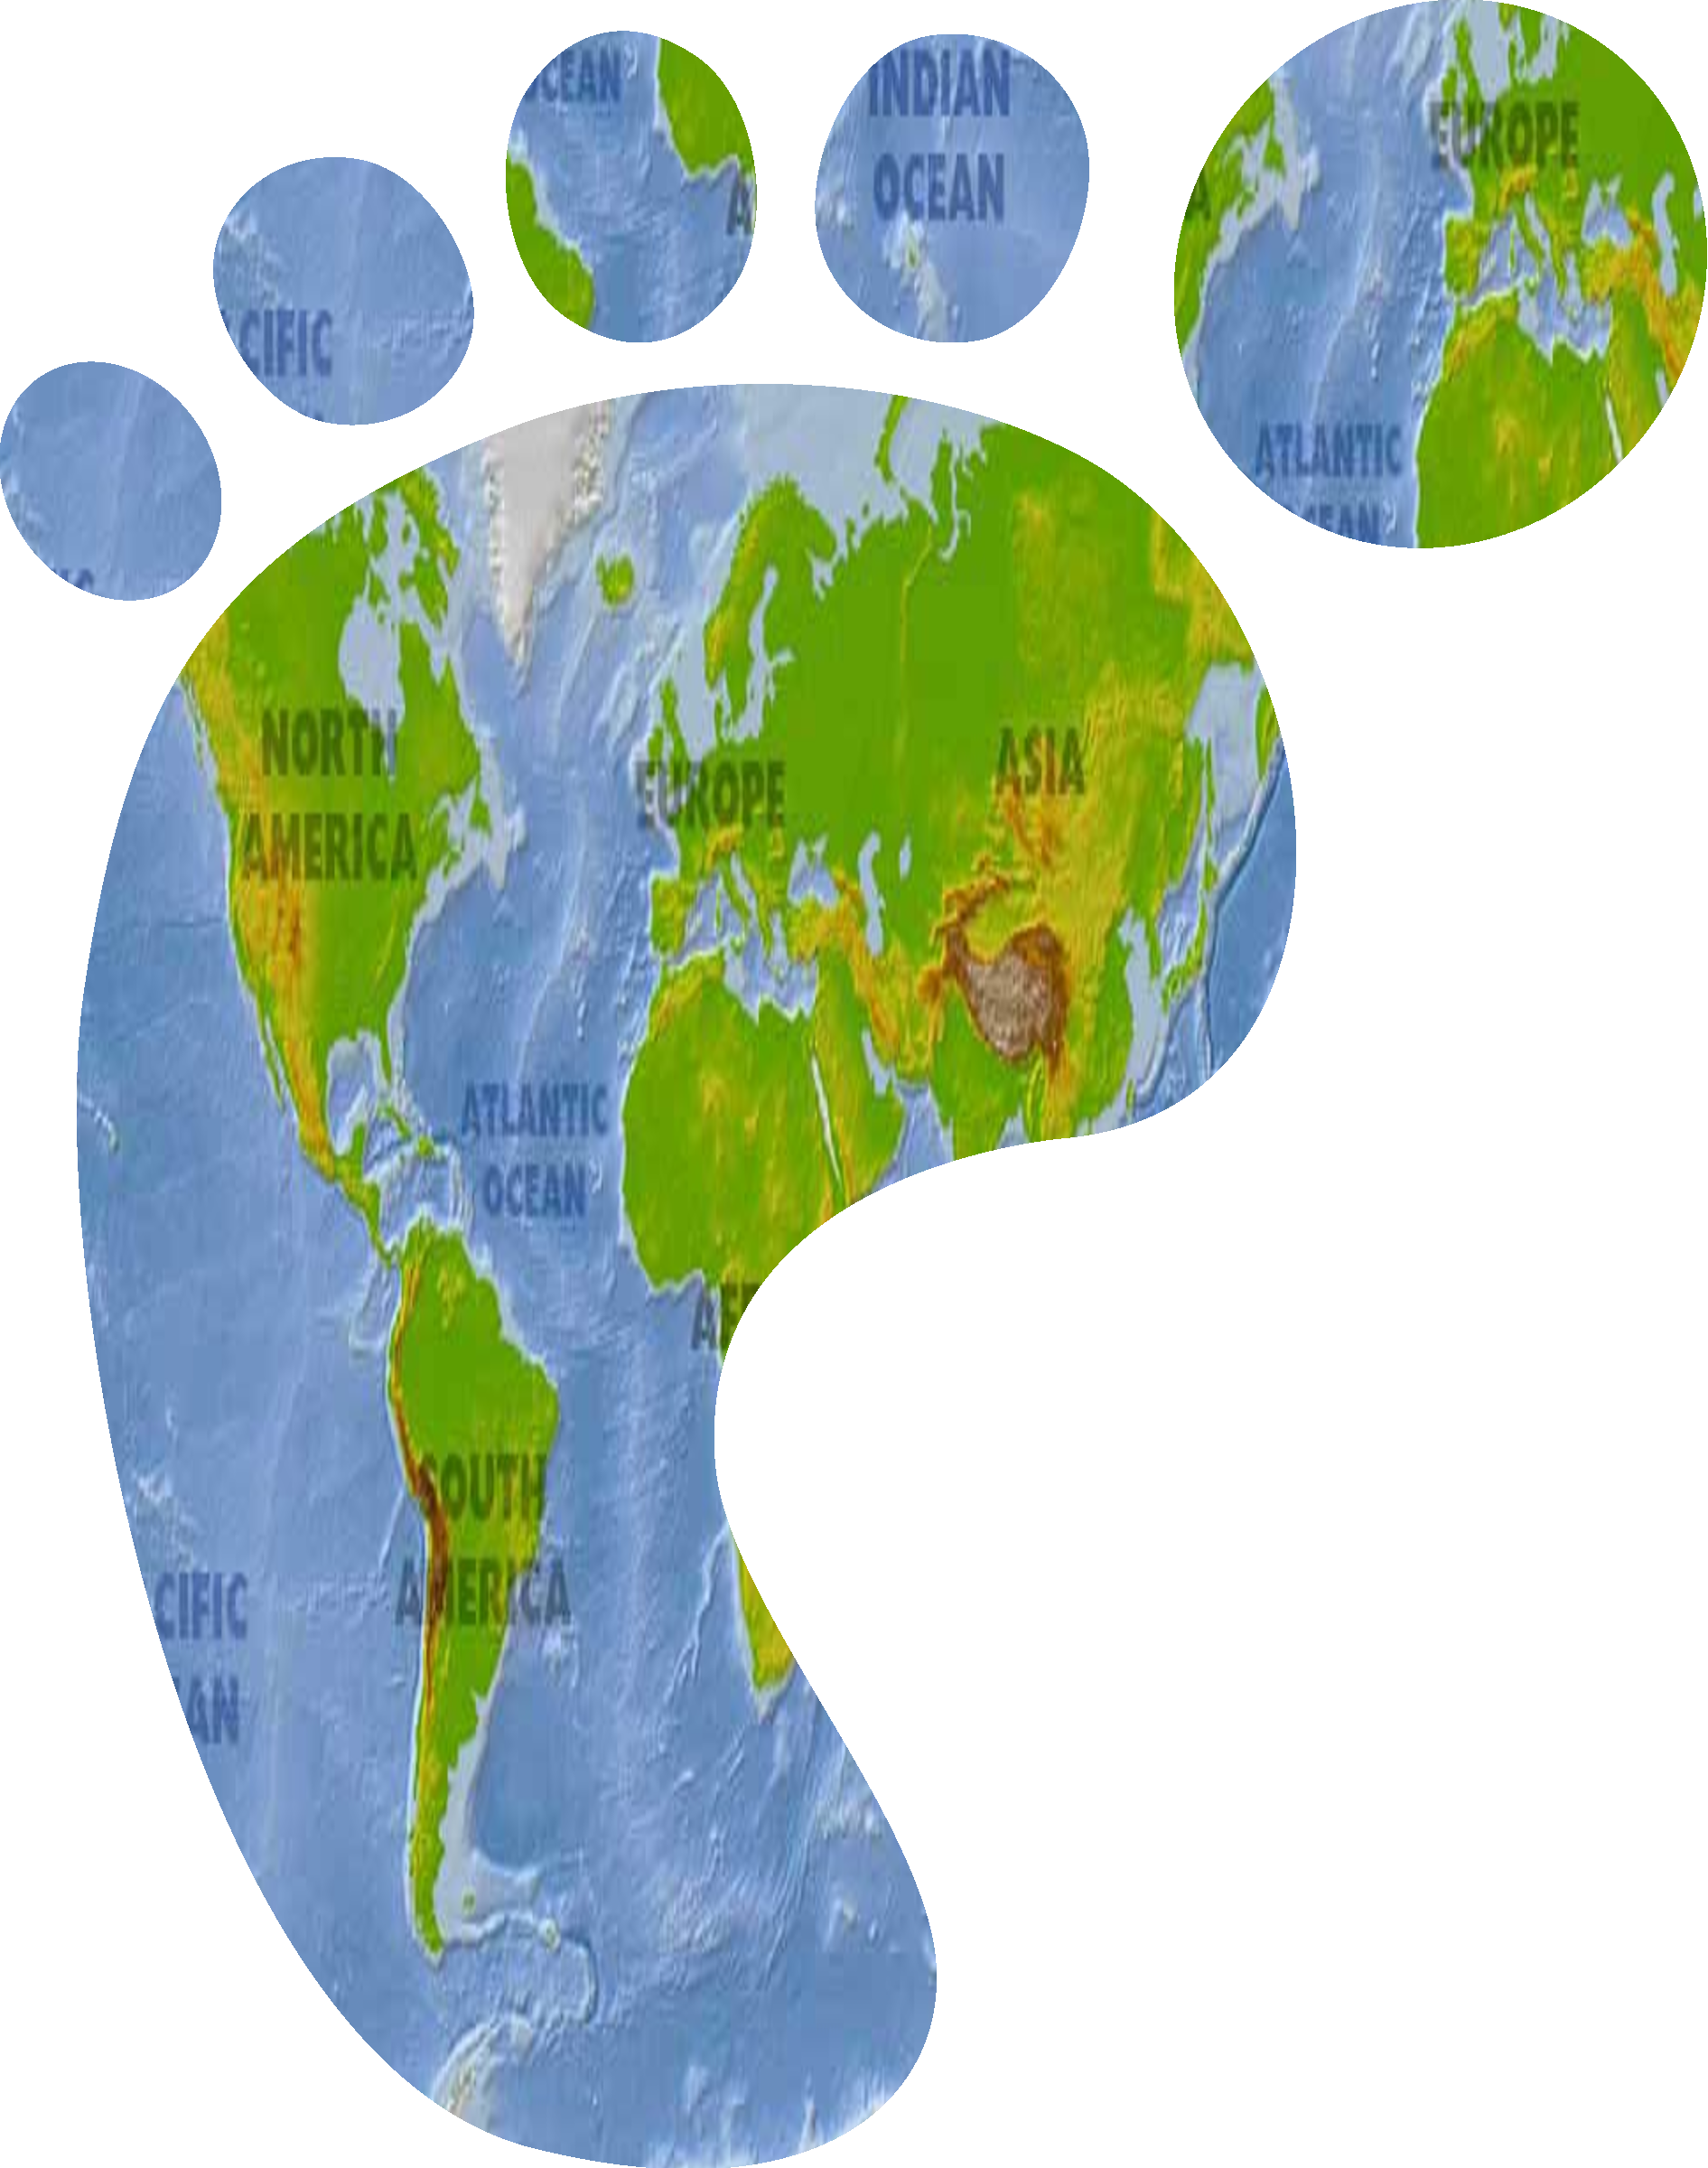
\includegraphics[width=0.4\textwidth]{./image/applogo.png}
\caption{\label{fig:login}Logo app}
\end{wrapfigure}

Partiamo da un presupposto fondamentale: l’interfaccia grafica di un’applicazione mobile, progettata e realizzata in modo che risulti il più possibile intuitiva e quindi “usabile” per gli utenti, è un fattore fondamentale per il successo dell’app stessa.\\ 
Da questo punto di vista è evidente che una maggiore usabilità si ottiene cercando di soddisfare le necessità più comuni degli utenti nel loro approccio con l’applicazione.
Per questo ho cercato di realizzare una user interface che sia davvero “vicina” alle esigenze dell'utilizzatore e sia quindi pensata per un uso agevole e intuitivo delle tecnologie mobile.\\

Una delle bestie nere di tutti i programmatori che può dare parecchio filo da torcere è l‘interfaccia grafica.\\ 
Su Android, nello specifico, gestire correttamente le dimensioni e il posizionamento degli elementi può essere veramente una grande rogna.\\

Anche la scelta dei colori è fondamentali, infatti i colori da me scelti sono :\\\\
\begin{itemize}
\item il blu che simboleggia pace, calma, tranquillità, comprensione, tolleranza, energia mentale e profondità di sentimenti, chi lo preferisce desidera situazioni serene, armonia ed intesa profonda nelle relazioni umane.\\
\item L'arancione che simboleggia energia e passione del rosso unito all'allegria, felicità e solarità del giallo.\\ 
Esso può rappresentare un' infinità di doti positive, attrazione, stimolo, il successo, ma anche il fascino.\\ 
Visto dall' occhio umano è un colore che dà la sensazione di calore, ma non è quel calore aggressivo e passionale del rosso. Parlando di abbigliamento, l'arancione ha un' ottima visibilità, delicatamente cattura l'attenzione, esaltando le parti più importanti del corpo. E' molto gradito dai giovani.\\
\end{itemize}

Le persone sembrano divise riguardo l’importanza delle icone. Da un lato abbiamo quelli che ritengono possa essere un’ottima strategia di marketing. Dopotutto, è la primissima cosa che l’utente vede della vostra app. Quando cercano qualcosa su App Store, lei è lì a cercare di ‘vendere‘ al meglio la vostra app mostrando la qualità ricercata nei dettagli.\\

Dall’altro lato, una volta che una semplice persona si trasforma in cliente e ha la vostra app sulla sua Home Screen, il proposito diventa all’improvviso differente. Gli utenti devono essere in grado di riconoscere la vostra app a colpo d’occhio, grazie all’icona.\\

Quindi ho scelto come icona (figura 3.6) un mondo a forma di piede ispirato sopratutto dal nome dell'applicazione "DiscountWalk" in quando l'app permette anche di risparmiare la strada da percorrere poichè il possessore dell'app sa già cosa vedere.\\

\chapter*{Conclusione}
\vspace{2em}
\markboth{Conclusione}{}
\addcontentsline{toc}{chapter}{Conclusione}

Nella tesi si è parlato di un'applicazione figlia del concetto di Marketing di prossimità che da la possibilità ad utenti di seguire dei percorsi e ricevere premi al raggiungimente dell'obiettivo minimo per ottenerli e agli operatori di creare percorsi e premi.\\

Tutto questo utilizzando la tecnologia android che si trova sulla maggior parte dei dispositivi al momento in circolazione e questa è anche uno degli elementi positivi dell'app.
Dato che il tempo permetteva la scelta di solo uno delle due grandi tecnologie che hanno più del 90\% dei dispositivi ho optato per svilluppare questa app in android invece di utilizzare swift.\\

L'applicazione descritta nella tesi si pone come potenziale strumento per incrementare il bacino clienterale dell'aziende che lo utilizzeranno con minimo sforzo dato che l'operatore dovrà solo creare percorsi e fornire dei premi ,tutto questo liberamente senza alcun limitazione.\\
Infatti l'operatore se adotta una buona strateggia di marketing potrà aumentare i suoi introiti fornendo ad esempio sconti su beni o servizi non molto richiesti.\\
Mentre per l'utente un applicazione del genere è una mano dal cielo dato che permette di avere già degli itinerari pronti e in più spinge quest'ultimo a visitare più obiettivi possibili al fine di ottenere i premi ad essi connessi.\\

Ma tutto questo io lo vedo solo come inizio di un'applicazione ben strutturato dal mio punto di vista sia implementativo che dal design e dalla semplicità di utilizzo.\\

La prima delle possibili estensioni è quella di rendere l'applicazione accessibile a tutte le piattaforme senza alcuna discriminazione e ancora altre possibili estensioni sono tante ad esempio si potrebbe aggiungere una sezione per permettere all'utente di commentare i percorsi , gli obiettivi , i premi e perchè no anche gli operatori , tutto questo sarebbe un bel salto in avanti dato che oramai si da un commento su tutto.\\
In più dato che numerosi studi sulla gamification hanno dichiarato che assicurano all'utente un'esperienza stimolante e soddisfacente tramite l'impegno, l'interesse e la partecipazione si potrebbe inserire una qualche forma di sfida che si può fare con un altro utilizzatore dell'app , tutto questo renderebbe più divertende l'utilizzo dell'applicazione da parte dell'utente e inoltre alla fine potrebbe portare a nuove amicizie mentre per l'operatore creare queste sfide porterebbe una pubblicità gratuita e nuovi clienti. 


\begin{thebibliography}{100}
\addcontentsline{toc}{chapter}{Bibliografia}
\bibitem{rif1} Negri, S. ,\emph{ “Il Marketing Di Prossimit\'a”, Universit\'a degli studi di Pisa, 2015.}\\[0.2cm]
\bibitem{rif2} DeLuca, K. (2015). , \emph{“Selling or Spying: The Legal Implications of Target Marketing
Through Geolocation Technologies”, Law School Student Scholarship, Paper 656,
2015, 2-28}\\[0.2cm]
\bibitem{rif3} Tussyadiah, I. P., \emph{“A concept of location-based Social Network Marketing”, Journal
of Travel Tourism Marketing, 29(3), 2012, 205-220.}\\[0.2cm]
\bibitem{rif4} Haines, E.,\emph{ “The dos and don’ts of proximity marketing in sponsorship”, Journal of Sponsorship, 2(2), 2009, 113-119.}\\[0.2cm]
\bibitem{rif5} Sciortino, F.S., \emph{“Gamification: uno strumento per il miglioramento della brand image di una citt`a e della sua attrattivit\'a turistica”, Universit\'a degli studi di Pisa, 2014.}\\[0.2cm]
\bibitem{rif6} Di Pierdomenico , P. \emph{ Proximity Marketing per la promozione del territorio , \url{http://www.argoserv.it/proximity-marketing-promozione-del-territorio}}\\[0.2cm]
\bibitem{rif7} Bucaresti, C., \emph{ “Applicazioni mobili in ambito turistico: stato dell’arte, tassonomia
e valutazione di casi di studio”, Universit`a di Bologna, 2014.}\\[0.2cm]
\bibitem{rif8} Ruzic, D., \emph{ Bilos, A., Kelic, I., “Development of mobile marketing in croatian tourism using location-based services”, Tourism and Hospitality Management, 2012, 151-159.}\\[0.2cm]

\bibitem{rif9}\url{https://www.jointag.com/2-grandi-brand-che-hanno-scelto-il-marketing-di-prossimita-mcdonald-e-carrefour/}\\


%\begin{thesitography}{100}
%\addcontentsline{toc}{chapter}{Siti consultati}

\bibitem{rif10}\url{http://www.linkedin.com/pulse/ibeacon-e-il-marketing-di-prossimit\%C3\%A0-carlo-finocchi?trk=seokp_posts_primary_cluster_res_title}\\

\bibitem{rif11}\url{https://www.jointag.com/il-museo-digitale-il-connubio-perfetto-tra-passato-e-futuro/}\\

\bibitem{rif12}\url{http://www.argoserv.it/proximity-marketing-promozione-del-territorio}\\

\bibitem{rif13}\url{http://www.ninjamarketing.it/2015/01/13/quicon-il-marketing-di-prossimita-col-cliente-al-centro-intervista/}\\

\bibitem{rif14} Denisi M. , \emph{"An integrated solution for proximity services with beacons" , 18 Dicembre 2014}\\[0.2cm]

\end{thebibliography}
%\end{thesitography}

\end{document}
